\chapter{Authorship attribution's tasks}

\epigraph{\textit{"Science is the systematic classification of experience."}\\George Henry Lewes}

The task of determining or verifying the authorship of an anonymous text based solely on internal evidence is a very old one, dating back at least to the medieval scholastics,
for whom the reliable attribution of a given text to a known ancient authority was essential to determining the text’s veracity. More recently, this problem of authorship attribution has gained greater prominence due to new applications in forensic analysis, humanities scholarship, and electronic commerce, and the development of computational methods for addressing the problem.
Statistical authorship attribution has a long history, culminating in the use of modern machine learning classification methods.
In the simplest form of the problem, we are given examples of the writing of a number of candidate authors and are asked to determine which of them authored a given anonymous
text. In this straightforward form, the authorship attribution problem fits the standard modern paradigm of a text categorization problem \cite{lewis1994comparison} \cite{sebastiani2002machine}. The components of text categorization systems are by
now fairly well understood: Documents are represented as numerical vectors that capture statistics of potentially relevant features of the text, and machine learning methods are
used to find classifiers that separate documents that belong to different classes.
In the next section we will briefly present the approach to this task in the era before machine learning. Later, we will discuss the different approaches of this particular task, whether to approach it as a profile-based or an instance-based problem, depending on which domain are we tackling: single-domain or cross-domain.
In the last section, we will introduce to the latest state of the art approaches for this particular classification task. 

\section{History of methodologies}

The first attempts to quantify the writing style go back to the 19th century, with the pioneering study of Mendenhall (1887) on the plays of Shakespeare, followed
by statistical studies in the first half of the 20th century by Yule (1938, 1944) and Zipf (1932) \cite{williams1975mendenhall} \cite{yule1938test} \cite{zipf1932selected}. Later, the detailed study by Mosteller and Wallace (1964) on the authorship of “The
Federalist Papers” (a series of 146 political essays written by John Jay, Alexander Hamilton, and James Madison, 12 of which claimed by both Hamilton and Madison) was undoubtedly the most influential work in authorship attribution \cite{stamatatos2009survey}. Their method was based on Bayesian statistical analysis of the frequencies of a small set of common words (e.g., “and,” “to,” etc.) and produced significant discrimination results between the candidate authors.
Essentially, the work of Mosteller and Wallace (1964) initiated nontraditional authorship attribution studies, as opposed to traditional human-expert-based methods. Since
then and until the late 1990s, research in authorship attribution was dominated by attempts to define features for quantifying writing style, a line of research known as \textit{“stylometry”} \cite{holmes1998evolution}. Hence, a great variety of measures, including sentence length, word length, word frequencies, character frequencies, and vocabulary richness functions, had been proposed. Rudman (1998) estimated that
nearly 1,000 different measures had been proposed by the late 1990s \cite{rudman1997state}. The authorship attribution methodologies proposed during that period were computer-assisted rather than
computer-based, meaning that the aim was rarely at developing a fully automated system. In certain cases, there were methods that achieved impressive preliminary results and
made many people think that the solution of this problem was too close.
The most characteristic example is the CUSUM (or QSUM) technique \cite{michaelson1990qsum} that gained publicity and was accepted in courts as expert evidence; however, the research community heavily criticized it and considered it generally unreliable \cite{holmes1995forensic}. Actually, the main problem of that early period was the lack of objective evaluation of the proposed methods. In most of the cases, the testing ground was literary works of unknown or disputed authorship (e.g., the Federalist Papers
case), so the estimation of attribution accuracy was not even possible. The main methodological limitations of that period concerning the evaluation procedure were the following:
\begin{itemize}
	\item The textual data were too long (usually including entire books) and probably not stylistically homogeneous.
	\item The number of candidate authors was too small (usually two or three).
	\item The evaluation corpora were not controlled for topic.
	\item The evaluation of the proposed methods was mainly intuitive (usually based on subjective visual inspection of scatterplots).
	\item The comparison of different methods was difficult due to lack of suitable benchmark data.
\end{itemize}

Since the late 1990s, things have changed in authorship attribution studies. The vast amount of electronic texts available through Internet media (e-mail messages, blogs, online
forums, etc.) have increased the need for efficiently handling this information. This fact had a significant impact in scientific areas such as information retrieval, machine learning,
and natural language processing (NLP). The development of these areas influenced authorship attribution technology as described:
\begin{itemize}
	\item Information retrieval research developed efficient techniques for representing and classifying large volumes of text.
	\item Powerful machine learning algorithms became available to handle multidimensional and sparse data, allowing more expressive representations. Moreover, standard evaluation
	methodologies have been established to compare different approaches on the same benchmark data.
	\item NLP research developed tools able to analyze text efficiently and provided new forms of measures for representing the style (e.g., syntax-based features).
\end{itemize}

More importantly, the plethora of available electronic texts revealed the potential of authorship analysis in various applications \cite{madigan2005author} in diverse areas including intelligence (e.g., attribution of messages or proclamations to known terrorists,
linking different messages by authorship) \cite{abbasi2005applying}, criminal law (e.g., identifying writers of harassing messages, verifying the authenticity of suicide notes) and
civil law (e.g., copyright disputes) \cite{chaski2005s}, and computer forensics (e.g., identifying the authors of source code of malicious software) \cite{frantzeskou2006effective} in addition to the traditional application to literary research (e.g., attributing anonymous or disputed literary works to known authors) \cite{burrows2002delta}. Hence, (roughly) the last decade can be viewed as a new era of authorship analysis technology, this time dominated by efforts to develop practical applications dealing with real-world texts (e.g., e-mail messages, blogs,
online forum messages, source code, etc.) rather than solving disputed literary questions. Emphasis has now been given to the objective evaluation of the proposed methods as well
as the comparison of different methods based on common benchmark corpora. In addition, factors playing a crucial role in the accuracy of the produced models are examined, such as the training text size \cite{marton2005compression}, the number
of candidate authors \cite{koppel2006authorship}, and the distribution of training texts over the candidate authors \cite{stamatatos2008author}.

\section{Training's approach}

In every authorship-identification problem, there is a set of candidate authors, a set of text samples of known authorship covering all the candidate authors (\textit{training corpus}), and a set of text samples of unknown authorship (\textit{test corpus}); each
one of them should be attributed to a candidate author. In this survey, we distinguish the authorship attribution approaches according to whether they treat each training text individually or cumulatively (per author). In more detail, some approaches concatenate all the available training texts per author in one big file and extract a cumulative representation of that author’s style (usually called the author’s profile) from
this concatenated text. That is, the differences between texts
written by the same author are disregarded. Such approach just described is called \textit{"profile-based approach"} and early work in authorship attribution has followed this practice \cite{mosteller2007inference}.
On the other hand, another family of approaches requires multiple training text samples per author to develop an accurate attribution model. That is, each training text is
individually represented as a separate instance of authorial style. Such \textit{"instance-based approaches"}\footnote{Note that this term should not be confused with instance-based learning methods\cite{mitchell1997artificial}} are described in the
next section, followed by hybrid approaches attempting to combine characteristics of profile-based and instance-based methods. We then compare these two basic approaches and
discuss their strengths and weaknesses across several factors.

\subsection{Profile-based approach}

One way to handle the available training texts per author is to concatenate them in one single text file. This large file is used to extract the properties of the author’s style. An unseen text is, then, compared with each author file, and the most likely author is estimated based on a distance measure. It should be stressed that there is no separate representation of each text sample but only one representation of a large file per author. As a result, the differences between the training texts by the same author are disregarded. Moreover, the stylometric measures extracted from the concatenated file may be quite
different in comparison to each of the original training texts.

\begin{figure}[ht]
	\centering
	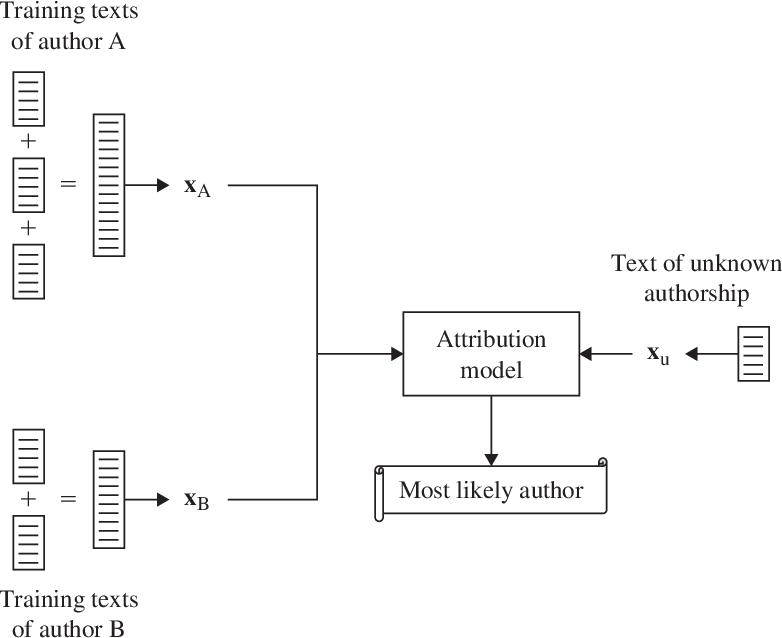
\includegraphics[width=.8\textwidth, height=.6\textheight, keepaspectratio]{profile-based-approach}
	\caption[Profile-based approach]{Typical architecture of profile-based in authorship attribution approaches \cite{stamatatos2009survey}}
	\label{fig:profile_based_approach}
\end{figure}

A typical architecture of a profile-based approach is depicted in figure  \ref{fig:profile_based_approach}. Note that $x$ denotes a vector of text representation
features. Hence, $x_A$ is the profile of Author $A$, and $x_u$ is the
profile of the unseen text.
The profile-based approaches have a very simple training process. Actually, the training phase just comprises the extraction of profiles for the candidate authors. Then, the attribution model is usually based on a distance function that computes the differences of the profile of an unseen text and the profile of each author. Let $PR(x)$ be the profile of text $x$ and $d[PR(x),PR(y)]$ the distance between the profile of text $x$ and the profile of text $y$. Then, the most likely author of an unseen text $x$ is given in \ref{autor_equation_1}, where $A$ is the set of candidate authors and $x_a$ is the concatenation of all training texts for author $a$.
\begin{equation}\label{autor_equation_1}
author(x) = \arg_{a \in A} min\ d(PR(x), PR(x_a)
\end{equation}


\subsection{Instance-based approach}

The majority of the modern authorship-identification approaches considers each training text sample as a unit that contributes separately to the attribution model. In other words, each text sample of known authorship is an instance of the problem in question. A typical architecture of such an instance-based approach is shown in figure  \ref{fig:instance_based_approach}. In detail, each text sample of the training corpus is represented by a vector of attributes $(x)$ following methods described earlier, and a
classification algorithm is trained using the set of instances of known authorship (\textit{training set}) to develop an attribution model. Then, this model will be able to estimate the true author of an unseen text.

\begin{figure}[ht]
	\centering
	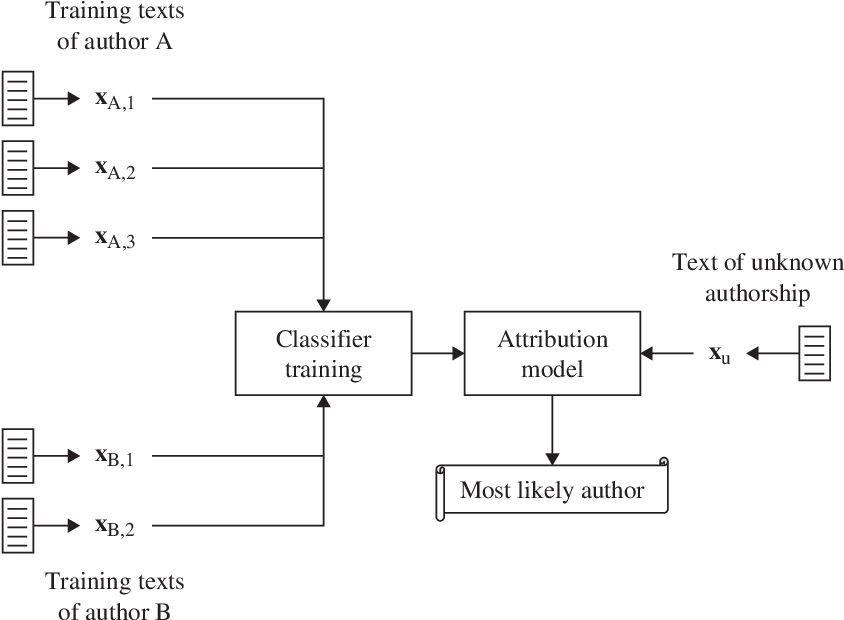
\includegraphics[width=.8\textwidth, height=.6\textheight, keepaspectratio]{instance-based-approach}
	\caption[Instance-based approach]{Typical architecture of instance-based in authorship attribution approaches \cite{stamatatos2009survey}}
	\label{fig:instance_based_approach}
\end{figure}

Note that such classification algorithms require multiple training instances per class for extracting a reliable model. Therefore, according to instance-based approaches, in case
we have only one, but a quite long, training text for a particular candidate author (e.g., an entire book), this should be segmented into multiple parts, probably of equal length.
From another point of view, when there are multiple training text samples of variable length per author, the training text instance length should be normalized. To that end, the training texts per author are segmented to equal-sized samples \cite{sanderson2006short}. In all these cases, the text samples should be long enough so that the text representation features can adequately represent their style. Various lengths of text samples have been reported in the literature. Sanderson and Guenter (2006) produced chunks of 500 characters \cite{sanderson2006short}. \citeauthor{koppel2006authorship} (\citeyear{koppel2006authorship}) segmented the training texts into
chunks of about 500 words \cite{koppel2006authorship}. \citeauthor{hirst2007bigrams} (\citeyear{hirst2007bigrams}) conducted experiments with text blocks of varying length (i.e.: 200, 500, and 1000 words) and reported significantly reduced accuracy as the text-block length decreases \cite{hirst2007bigrams}. Therefore, the choice of the training instance text sample is not a trivial process and directly affects the performance of the attribution model.


\section{The real problem}

Statistical authorship attribution has a long history, culminating in the use of modern machine learning classification methods. Nevertheless, most of this work suffers from the limitation of assuming a small closed set of candidate authors and essentially unlimited training text for each. Real-life authorship attribution problems, however, typically fall short of this ideal. Thus in \cite{koppel2009computational} three scenarios are presented for which solutions to the basic attribution problem are inadequate.
For example, we may encounter scenarios such as:

\begin{enumerate}
	\item There is no candidate set at all. In this case, the challenge is to provide as much demographic or psychological information as possible about the author. This is the \textit{profiling problem}.
	\item There are many thousands of candidates for each of whom we might have a very limited writing sample. This is the \textit{needle-in-a-haystack} problem.
	\item There is no closed candidate set but there is one suspect. In this case, the challenge is to determine if the suspect is or is not the author. This is the \textit{verification problem}.
\end{enumerate}

In the following section we will show how machine learning methods can be adapted to handle the special challenges of each variant.

\subsection{Profiling problem}
Even in cases where we have an anonymous text and no candidate authors, we would like to say something about the anonymous author. That is, we wish to exploit the sociolinguistic observation that different groups of people speaking or writing in a particular genre and in a particular language use that language differently \cite{chambers2004handbook}.
This authorship profiling problem is of growing importance in the current global information environment applications abound in forensics, security, and commercial settings. For example, authorship profiling can help police identify characteristics of the perpetrator of a crime when there are too few (or too many) specific suspects to consider. Similarly, large corporations may be interested in knowing what types of people like or dislike their products, based on analysis of blogs and online product reviews. The question we therefore ask is: How much can we discern about the author of a text simply by analyzing the text itself? It turns out that, with varying degrees of accuracy, we can say a great deal indeed.
One of the approach to authorship profiling is to apply machine learning to text categorization. The process is as follows: First, we take a given corpus of training documents, each labeled according to its category for a particular profiling dimension. For example, when addressing classification by author gender, training documents are labeled as either \textit{male} or \textit{female}. Each document is then processed to produce a numerical vector, each of whose elements represents some feature of the text that might help discriminate the relevant categories. A machine learning method then computes a classifier that, to the extent possible, classifies the training examples correctly. Finally, the predictive power of the classifier is tested on out-of-training data.
Essentially the same paradigm can be used for authorship attribution, where the training texts are known writings of given candidate authors.\cite{juola2008authorship}

\subsection{Needle-in-hay-stack problem}

Consider now the scenario where we seek to determine the specific identity of a document’s author, but there are many thousands of potential candidates. We call this the \textit{needle-in-a-haystack} attribution problem. In this case, standard text-classification techniques are unlikely to give reasonable accuracy and may require excessive computation time to learn classification models; however, in \cite{koppel2009computational} and \cite{koppel2011authorship} state that if we are willing to tolerate our system telling us it does not know the answer, we can achieve high accuracy for the cases where the system does give us an attribution it consider reliable.
Recent works, \cite{schwartz2013authorship} and \cite{theophilo2019needle} have addressed the problem with tackling a large set of candidate authors while keeping the documents very short, also known as "micro-messages" or "tweets"\footnote{As the name recall, the name of the posts on the popular social media platform Twitter. Its main characteristics is that originally only 140 characters per post were allowed (at the moment of writing, it has been upgraded up to 280 characters per tweet).}.

\subsection{Verification problem}
 
Considering the case in which we are given examples of the writing of a single author and are asked to verify that a given target text was or was not written by this author. As a categorization problem, verification is significantly more difficult than basic attribution, and virtually no work has been done on it (but see \citeauthor{halteren2004linguistic} \citeyear{halteren2004linguistic}), outside the framework of plagiarism detection \citeauthor{zu2007plagiarism} \citeyear{zu2007plagiarism}. If, for example, all we wished to do is to determine if a text had been written by Shakespeare or by Marlowe, it would be sufficient to use their respective known writings, to construct a model distinguishing them, and to test the unknown text against the model. If, on the other hand, we need
to determine if a text was written by Shakespeare, it is difficult to assemble a representative sample of non-Shakespeare texts.
The situation in which we suspect that a given author may have written some text, but do not have an exhaustive list of alternative candidates, is a common one \cite{koppel2009computational}. The problem is complicated by the fact that a single author may vary his or her style from text to text or may unconsciously drift stylistically over time, not to mention the possibility of conscious deception. Thus, we must learn to somehow distinguish between relatively shallow differences that reflect conscious or unconscious changes in an author’s style and deeper differences that reflect styles of different authors.

\section{Identify the problem}

Since authorship attribution has been studied for many decades now, we have witnessed the rise of many different subtasks. In the next part of this section we will illustrate one of the main difference between approaching a single domain or a cross domain dataset in order to get the stylometric markers of each authors.
We will also discuss the difference between closed set and open set authorship attribution problem.

\subsection{Single domain vs Cross domain}

When dealing with a dataset with documents written by different authors, the first analysis to carry is to identify the different topics of each document written by the same author. This analysis is very important for the rest of the analysis, because previous works have shown a degradation in terms of performance when approaching cross domain dataset, being suited for the single domain approach.
The reason behind this is trivial: content words used by the same author will vary a lot when writing about different topics (such as: motors, science, literature,or politics). What should remain steady in the style of writing of an author across different topics should be function words, the use of punctuation ..etc
Although a lot of work showed good results in both context (\cite{sapkota2015not}, \cite{kestemont2019overview}, \cite{overdorf2016blogs}) for the rest of this work, we will focus on single domain authorship attribution, but we will also show results of our model trained on a cross domain dataset\footnote{\textit{The Guardian}, described in chapter 4}. 

\subsection{Closed set vs Open set}

The simplest kind of authorship attribution problem—and the one that has received the most attention—is the one in which we are given a small closed set of candidate authors and are asked to attribute an anonymous text to one of them. Usually, it is assumed that we have copious quantities of text by each candidate author and that the anonymous text is reasonably long. A number of recent survey papers amply cover the variety of methods used for solving this problem, known as \textit{closed set authorship attribution}.\\
A significant fact that examination of the literature reveals is that nearly all research in the field only considers the simplest version of the problem.\\\\
Unfortunately, this “vanilla” version of the authorship attribution problem does not often arise in the real world. We often encounter situations in which our list of candidates might be very large and in which there is no guarantee that the true author of an anonymous text is even among the candidates. \cite{koppel2012fundamental}
Similarly, almost all work in authorship attribution has focused on the case in which the candidate set is a closed set—the anonymous text is assumed to have been written by one of the known candidates. The more general case, in which the true author of an anonymous text might not be one of the known candidates, reduces to the binary authorship verification problem: determine if the given document was written by a specific author or not.
Some references of works tackling open set authorship attribution problem are shown in \citeauthor{koppel2011authorship} (2011) and in \citeauthor{badirli2019open} (2019).
However, we decided to focus our work in tackling the closed set authorship attribution problem, but we will leave some thoughts for future work in the correspondent chapter.